\documentclass[conference]{IEEEtran}
\IEEEoverridecommandlockouts
% The preceding line is only needed to identify funding in the first footnote. If that is unneeded, please comment it out.
\usepackage{cite}
\usepackage{amsmath,amssymb,amsfonts}
\usepackage{algorithmic}
\usepackage{graphicx}
\usepackage{textcomp}
\usepackage{xcolor}
\def\BibTeX{{\rm B\kern-.05em{\sc i\kern-.025em b}\kern-.08em
    T\kern-.1667em\lower.7ex\hbox{E}\kern-.125emX}}
\begin{document}

\title{Weather386}

\author{
  \IEEEauthorblockN{Taylor Davis}
  \IEEEauthorblockA{\textit{Statisitcs, BYU.} \\
  \textit{Provo, USA} \\
  tpd25@student.byu.edu}
  \and
  \IEEEauthorblockN{Cameron Slaugh}
  \IEEEauthorblockA{\textit{Statistics, BYU.} \\
  \textit{Provo, USA} \\
  cmslaugh@student.byu.edu}
}

\maketitle

\begin{abstract}
    Weather386 is a Python project developed as part of a Stat 386 at Brigham Young University with the aim of providing a user-friendly interface for accessing and visualizing both weather forecast and historical data and being able to compare them. This package simplifies the process of retrieving and analyzing weather information from the National Weather Service, offering a range of functions for ease of use. All timestamps within the package adhere to the UTC timezone, in accordance with standard practices for weather data. This report outlines the key functionalities of Weather386 and its application in obtaining and visualizing weather forecasts and historical data. For the most part, data collected from Kansas City showed that the forecast was greater than the average.
\end{abstract}

\begin{IEEEkeywords}
weather, location, normal, temperature, wind speed, precipitation
\end{IEEEkeywords}

\section{Introduction}
    In the realm of data science, the efficient extraction and analysis of data play a pivotal role. Weather386 addresses this need by providing a Python package designed for simplicity and effectiveness in analyzing weather data. The package facilitates access to weather forecast and historical data from the National Weather Service through straightforward functions. This report introduces Weather386, highlighting its purpose, utility, and how it was used to compare recent data in the Kansas City Area.

\section{Methods}
    To discover if weather in Kansas City would be normal or abnormal we created several functions to help with the cleaning and visualization of weather forecast and their significance. For example, obtaining a weather forecast involves creating necessary functions such as get_forecast, get_history, join_clean to pull the data from their databases and compile it into a neat data set. Latitude and longitude measurements define the geographical location of interest, and these can be specified based on user requirements. A practical usage example is provided, demonstrating the step-by-step process of fetching a weather forecast, obtaining historical data, and cleaning the forecast dataframe. In addition to this a combined_graph function was made to generate graphs for precipitation, temperature, and Wind Speed every 4 hours for a week. These graphs showed the historical average along with its confidence interval and overlaid the forcast for that week to see if the forcast was normal or abnormal. When running these functions in sync, we get the following graphs which we used in our analysis.

\begin{figure}[htbp]
    \centerline{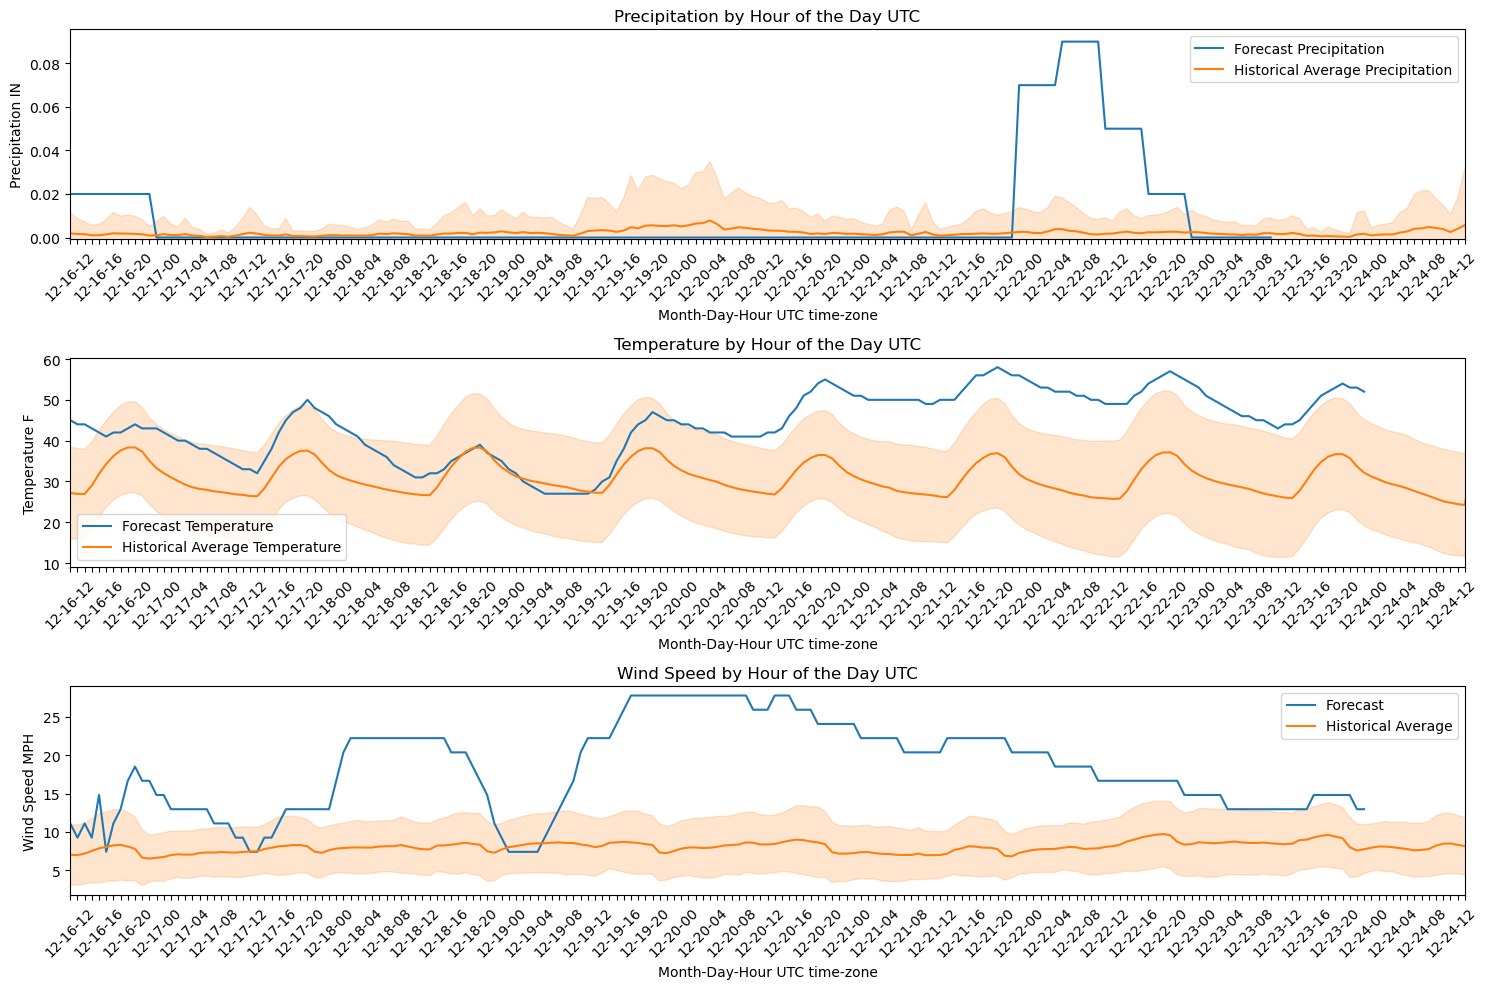
\includegraphics{example_graph.png}}
    \caption{Example of a figure caption.}
    \label{fig}
    \end{figure}

\section{Results}
Precipitation Analysis
The graphical representation provides valuable insights into anticipated weather conditions. Notably, the forecast indicates a significant likelihood of precipitation on the 22nd, suggesting an anomalous weather event for this particular day in December. This information is crucial for planning and preparedness, as it highlights a deviation from typical weather patterns.

Temperature Trends
Examining the temperature graph reveals consistent temperatures ranging from 30 to 45 degrees, reflective of seasonal norms. However, a distinctive shift is observed starting on the 20th, indicating an impending period of uncharacteristically warm weather for this time of year. This deviation is noteworthy, emphasizing the importance of visualizing temperature trends to identify and understand unusual weather phenomena.

Wind Speed Analysis
The forecasted wind speeds present a notable departure from the norm throughout the forecast period. Particularly noteworthy is the expectation of heightened wind activity on the 20th, with speeds reaching up to 30 mph—approximately 20 mph above the customary levels for this season. This insight into elevated wind conditions underscores the significance of considering not only precipitation and temperature but also factors like wind speed when assessing weather forecasts.

\section{Conclusion}
In conclusion, Weather386 is a valuable tool for data scientists and weather enthusiasts seeking a seamless approach to accessing and visualizing weather data. This Python package prioritizes simplicity, offering users an intuitive interface for interacting with the National Weather Service's vast database of forecast and historical information. As demonstrated in the usage example, Weather386 streamlines the process of data retrieval and analysis, presenting users with clean, actionable data and insightful visualizations. The package's utility extends to diverse applications, making it a versatile asset for those engaging in weather-related data science projects.

\begin{thebibliography}{00}
\bibitem{b1} Zippenfenig, Patrick. Open-Meteo.com Weather API., Zenodo, 2023, doi:10.5281/ZENODO.7970649.
\bibitem{b2} Hersbach, H., Bell, B., Berrisford, P., Biavati, G., Horányi, A., Muñoz Sabater, J., Nicolas, J., Peubey, C., Radu, R., Rozum, I., Schepers, D., Simmons, A., Soci, C., Dee, D., Thépaut, J-N. (2023). ERA5 hourly data on single levels from 1940 to present [Data set]. ECMWF. https://doi.org/10.24381/cds.adbb2d47
\bibitem{b3} Muñoz Sabater, J. (2019). ERA5-Land hourly data from 2001 to present [Data set]. ECMWF. https://doi.org/10.24381/CDS.E2161BAC
\bibitem{b4} Schimanke S., Ridal M., Le Moigne P., Berggren L., Undén P., Randriamampianina R., Andrea U., Bazile E., Bertelsen A., Brousseau P., Dahlgren P., Edvinsson L., El Said A., Glinton M., Hopsch S., Isaksson L., Mladek R., Olsson E., Verrelle A., Wang Z.Q. CERRA Sub-Daily Regional Reanalysis Data for Europe on Single Levels from 1984 to Present. ECMWF, 2021, doi:10.24381/CDS.622A565A.
\bibitem{b5} https://api.weather.gov https://www.weather.gov/documentation/services-web-api
\end{thebibliography}

\end{document}
